\documentclass[12pt]{article}

\usepackage[a4paper,margin=2cm]{geometry}
\usepackage{amsmath, amssymb, amsthm, amsfonts, tikz, algpseudocode}
\usepackage[plain]{algorithm}
\usepackage[framemethod=TikZ]{mdframed}
\definecolor{newblue}{rgb}{0.2,0.2,0.6}
\usepackage{caption}
\usepackage{graphicx}
\usepackage{float}
\usepackage{listings}
\usepackage{color}
\usepackage{xcolor}
\usepackage[colorlinks,allcolors=newblue]{hyperref}
\usepackage{listings}
\lstset{
    basicstyle=\scriptsize\ttfamily,
    commentstyle=\ttfamily\color{gray},
    numbers=left,
    numberstyle=\ttfamily\color{gray}\footnotesize,
    stepnumber=1,
    numbersep=5pt,
    backgroundcolor=\color{white},
    showspaces=false,
    showstringspaces=false,
    showtabs=false,
    frame=single,
    tabsize=2,
    captionpos=b,
    breaklines=true,
    breakatwhitespace=false,
    title=\ttfamily\lstname,
    escapeinside={},
    keywordstyle={},
    morekeywords={}
}

\input{config/lecture-header}
\input{config/math-boxes}

\definecolor{dfn-color}{rgb}{0,0.48,0.65}


\begin{document}
\lecture{Introduction}{January 11, 2018}{Dev Dabke}

\section{Logistics}\label{sec:logistics}

\begin{info}[Contact Information]{info:contact}
    \begin{itemize}
        \item Email address: \href{mailto:dv@math.duke.edu}{dv@math.duke.edu}
        \item Office Hours: To Be Determine, By Appointment
        \item Course Slack: \href{cattheory.slack.com}{cattheory.slack.com}
    \end{itemize}
\end{info}

\begin{info}[Course Structure]{info:structure}
    \begin{itemize}
        \item 50\% of grade: \( \approx 7 \) problem sets in \LaTeX
        \item 1 course project
        \item Some use of Haskell
    \end{itemize}
\end{info}

\section{Basic Definitions}\label{sec:definitions}

We will take the definition of a set for granted and we will assume the use of naive set theory.
Additionally, we assume the notion of a function (or map) and the standard notation for an application of a function \( f(\ldots) \).
Finally, we assume basic logic, like ``and'' and ``or'' operators.
Moreover, we may use the symbols of ``logical or'' \( \lor \) and ``logical and'' \( \land \).

\begin{dfn}[Relation]{dfn:relation}
    On some set \( X \), a \textcolor{dfn-color}{binary relation} is a function \( \textcolor{dfn-color}{\sim} \) such that
    \[
        \sim \, : X \times X \to \mathbb{B}
    \]
    where \( \mathbb{B} = \{ \top, \bot \} \).
    Where \( x_1, x_2 \in X \), we write \( x_1 \sim x_2 \) to mean \( \sim(x_1, x_2) = \top \).
    \\ \\
    In other words, a relation is a ``binary'' or ``2-ary'' function (i.e.\ it takes two inputs) and returns either a true or false value (also notated as a \( 1 \) or \( 0 \)).
\end{dfn}

\begin{dfn}[Pre-Order]{dfn:pre-order}
    A \textcolor{dfn-color}{pre-order} \( (P, \textcolor{dfn-color}{\leq}) \) is a set \( P \) with a \hyperref[dfn:relation]{binary relation} \( \leq \) such that
    \begin{itemize}
        \item \( \forall x \in P, \, x \leq x \) (reflexivity)
        \item \( \forall x, y, z \in P, \, [x \leq y \text{ and } x \leq z] \implies x \leq z \) (transitivity)
    \end{itemize}
    We also say that \( x \) \textcolor{dfn-color}{precedes} \( y \) when \( x \leq y \).
    \\ \\
    If \( \leq \) satisfies the condition that
    \[
        \forall x, y \in P, \, [x \leq y \text{ and } y \leq x] \implies x = y
    \]
    then we say that \( P \) is a \textcolor{dfn-color}{partially ordered set}.
    \\ \\
    If \( \leq \) satisfies the condition that
    \[
        \forall x, y \in P, \, x \leq y \text{ or } y \leq x
    \]
    then we say that \( P \) is a \textcolor{dfn-color}{totally ordered set}.
\end{dfn}

\begin{dfn}[Bijection, Bijective]{dfn:bijection}
    A function or map \( f : X \to Y \) is \textcolor{dfn-color}{bijective} or \textcolor{dfn-color}{a bijection} if \( \exists g : Y \to X \) such that
    \begin{align*}
        f(g(y)) &= y \\
        g(f(x)) &= x
    \end{align*}
    for all \( y \in Y \) and \( x \in X \).
    \\ \\
    For a bijection \( f \), we may write
    \[
        f : X \xrightarrow{\textcolor{dfn-color}{\cong}} Y
    \]
\end{dfn}

\begin{dfn}[Pre-Image]{dfn:pre-image}
    Of a function \( f : X \to Y \), the \textcolor{dfn-color}{pre-image} \( f^{\textcolor{dfn-color}{-1}} \) is the set
    \[
        f^{-1} (B) = \{ x \in X : f(x) \in B \}
    \]
\end{dfn}

\section{Working with Pre-Orders}\label{sec:working-with-pre-orders}

\begin{eg}[Pre-Order with Power Sets]{eg:powerset}
    Let \( X = \{ a, b, c \} \), i.e.\ a set with elements \( a, b, c \).
    We say that its powerset \( \mathcal{P}_{X} \) consists of all subsets of \( X \) (which includes \( X \) itself and the empty set).
    We will construct the \hyperref[dfn:pre-order]{pre-order} \( (\mathcal{P}_{X}, \subseteq) \) of set inclusion.
    \\ \\
    Associated to this pre-order, we can draw the following diagram
    \\ \\
    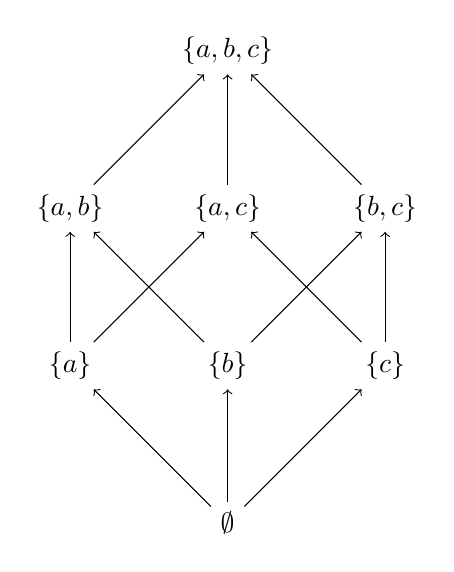
\begin{tikzpicture}[node distance=2cm]
        \node (empty) {\( \emptyset \)};

        \node (b) [above of=empty] {\( \{ b \} \)};
        \node (a) [left of=b] {\( \{ a \} \)};
        \node (c) [right of=b] {\( \{ c \} \)};

        \node (ac) [above of=b] {\( \{ a, c \} \)};
        \node (ab) [left of=ac] {\( \{ a, b \} \)};
        \node (bc) [right of=ac] {\( \{ b, c \} \)};

        \node (abc) [above of=ac] {\( \{ a, b, c \} \)};

        \path[->,scale=3]
            (empty) edge node [above] {} (a)
            (empty) edge node [above] {} (b)
            (empty) edge node [above] {} (c)

            (a) edge node [above] {} (ab)
            (a) edge node [above] {} (ac)
            (b) edge node [above] {} (ab)
            (b) edge node [above] {} (bc)
            (c) edge node [above] {} (ac)
            (c) edge node [above] {} (bc)

            (ab) edge node [above] {} (abc)
            (ac) edge node [above] {} (abc)
            (bc) edge node [above] {} (abc)
        ;
    \end{tikzpicture}
    \\ \\
    where \( \longrightarrow \) denotes set inclusion.
    Importantly, we are only denoting some arrows.
    However, since the pre-order has the transitive property, we simply have to denote a ``covering'' set of \( \longrightarrow \), which we have done.
    In other words: all subset relationships are represented by \( \longrightarrow \) or some sequence of \( \longrightarrow \)s.
\end{eg}

\begin{dfn}[Greatest, Least Elements; Top, Bottom]{dfn:el-great}
    Given some \hyperref[dfn:pre-order]{pre-order} \( (P, \leq) \), we say that
    \begin{alignat*}{3}
        x \in P \text{ is a }
        &\text{\textcolor{dfn-color}{greatest}} \text{ element or }
        &\text{\textcolor{dfn-color}{top}} \hspace{1cm} \text{ if }
        &y \leq x \, \forall y \in P \\
        &\text{\textcolor{dfn-color}{least}} &\text{\textcolor{dfn-color}{bottom}} \hspace{1cm}
        &x \leq y
    \end{alignat*}
\end{dfn}

\begin{prp}[Binary Encoding Map]{prp:binary-encoding-map}
    Given some set \( X \), all \( A : A \subseteq X \) correspond to some map \( \epsilon_{A} : X \to \mathbb{B} \).
\end{prp}

\begin{eg}[Binary Encoding Map]{eg:binary-encoding-map}
    Let \( X = \{ a, b, c \} \) and \( A = \{ a, c \} \).
    Then the corresponding encoding map \( \epsilon_{A} \) can be defined as
    \[
        \epsilon_{A}(x) \triangleq
        \begin{cases}
            \top = 1 & x = a \\
            \bot = 0 & x = b \\
            \top = 1 & x = c
        \end{cases}
    \]
    for \( x \in X \).
\end{eg}

\begin{prp}[Set Inclusion Map]{prp:set-inclusion-map}
    For some set \( X \) and its \hyperref[eg:powerset]{powerset} \( \mathcal{P}_{X} \), \( \exists f \) such that
    \begin{align*}
        f : \mathcal{P}_{X} &\xrightarrow{\cong} \mathcal{B} \\
        A &\mapsto
        \left [
            x \mapsto
            \begin{cases}
                \top & x \in A \\
                \bot & x \notin A \\
            \end{cases}
        \right]
    \end{align*}
    where \( \mathcal{B} \) is the set of all maps \( f \) such that \( f : X \to \mathbb{B} \).
\end{prp}

\begin{prf}[Proof of Proposition~\ref{prp:set-inclusion-map}]{prf:set-inclusion-map}
    We proceed with a constructive proof by constructing \( g \) such that
    \begin{align*}
        g : \mathcal{B} &\to \mathcal{P}_{X} \\
        \phi &\mapsto \phi^{-1}(\top)
    \end{align*}
    We can now check the definition of a \hyperref[dfn:bijection]{bijection}.
    We check the forward direction and note that
    \begin{align*}
        g(f(A)) &= g
        \left(
            x \mapsto
            \begin{cases}
                \top & x \in A \\
                \bot & x \notin A \\
            \end{cases}
        \right) \\
        &= \{ x : x \in A \} \\
        &= A
    \end{align*}
    Checking the backwards direction yields
    \begin{align*}
        f(g(\phi)) &= f\left( \phi^{-1}(\top) \right) \\
        &= x \mapsto
            \begin{cases}
                \top & x \in \phi^{-1}(\top) \\
                \bot & x \notin \phi^{-1}(\top) \\
            \end{cases} \\
        &= \phi
    \end{align*}
\end{prf}

\section{Special Subsets and their Pre-Order}\label{sec:subsets}

\begin{dfn}[Union, Intersection]{dfn:union-intersection}

\end{dfn}

\end{document}
